\section{Аналитическая часть}
 
Транслятор --- программа или техническое средство, выполняющие трансляцию программы. \cite{translate}
 
Трансляция программы --- преобразование программы, представленной на одном языке программирования, в программу на другом языке и в определенном смысле равносильную первой. \cite{translate}
 
Статическая трансляция (Ahead-of-time (AOT)) --- трансляция проводящаяся до начала выполнения программы. Позволяет использовать более трудозатратные методы оптимизации.

Динамическая трансляция (Just-in-time (JIT)) --- трансляция выполняемая непосредственно во время выполнения программы. Имеет строгие ограничения на скорость трансляции.

Интерпретация --- построчный анализ, обработка и выполнение кода программы, в отличие от компиляции, где весь текст программы, перед запуском анализируется и транслируется в машинный или байт-код без её выполнения. \cite{interpret}
 
Блок трансляции --- непрерывная последовательность инструкций программы выделенная для трансляции.
 
Промежуточное представление ---  это специальный код используемый внутри компилятора или виртуальной машины для представления исходного кода. Предназначен для дальнейшей обработки, такой как оптимизация и трансляция в машинный код.
 
Статическое единственное присваивание (СЕП) --- промежуточное представление в котором каждой переменной значение присваевается один раз, переменные исходной программы разбиваются на версии, обычно с помощью добавления суффикса, таким образом, что каждое присваивание осуществляется уникальной версии переменной.
  
Трансляция машинных кодов решает задачу запуска программ собранных под иную, по отношению к запускающей машине, архитектуру. При динамической трансляции существуют следующие проблемы:

\begin{itemize}[leftmargin=1.6\parindent]
	\item[---] выделение регистров;
	\item[---] поддержка самоизменяемого кода;
	\item[---] корректная трансляция;
	\item[---] быстрая трансляция;
	\item[---] сохранение скорости выполения кода.
\end{itemize}

Последние два пункта, при динамической трансляции, представляют собой смежные проблемы. Действительно, если применить все возможные оптимизации оптимизирующего компилятора LLVM к блоку трансляции этот блок будет выполнятся на сравнимой с изначальной скорости. Однако проходы оптимизации займут непозволительно большое время, что в итоге приведет к замедлению выполнения кода, нахождение этого баланса и является главной проблемой динамической трансляции. 

\subsection{Существующие решения}

Рассматриваются QEMU, box64 и FEX.

\subsection{Трансляция}

Все рассматриваемые проекты поддерживают динамическую трансляцию для архитектуры ARM. Два из них --- QEMU и FEX --- поддерживают промежуточное представление. FEX поддерживает плохо оптимизированную трансляцию в x86 (в основном для отладки), box64 включает в себя эмулятор написанный на C, его можно воспринимать как интерпретатор, он используется при запуске на любой архитектуре кроме ARM.

В box64 не используеются промежуточное представление, таким образом при динамической рекомпиляции поддерживаемые инструкции, при помощи макросов C, транслируются в инструкции ARM.

В QEMU в качестве промежуточного представления используются «TCG ops» по организации похожие на инструкции архитектур RISC.

В FEX в качестве промежуточного представления используются СЕП инструкции напоминающие ARM. Использование СЕП облегчает оптимизацию кода, например при устранении бессмысленных присвоений:\\
\texttt{y := 1\\
	y := 2\\
	x := y}

Не сложно понять что первое присвоение переменной не нужно, однако для транслятора это далеко не так очевидно, при использовании SSA:\\
\texttt{y1 := 1\\
	y2 := 2\\
	x1 := y2\\}
такую ситуацию проще отследить. 

В целом SSA помогает с:
\begin{itemize}[leftmargin=1.6\parindent]
	\item[---] свёрткой констант;
	\item[---] удалением мёртвого кода;
	\item[---] частичным устранением избыточности;
	\item[---] снижением стоимости операций;
	\item[---] распределением регистров.
\end{itemize}

\subsection{QEMU}

кему это круто написать что это такое \cite{qemu}

\subsubsection{Сворачивание и оптимизация тривиальных выражений}

В qemu определены свое промежуточное представление называющееся TCG ops, эти операции сначала оптимизируются, а затем выполняются на хосте, таким образом проще портировать TCG на разные платформы. Операции поддерживаются над 32 и 64 битными целыми числами, указатели определены как алиас над соответствующим целым числом.

Пример операции TCG:\\
\texttt{add\_i32 t0, t1, t2  (t0 <- t1 + t2)}

Одной из оптимизаций является игнорирование бессмысленных операций, например операция:\\
\texttt{and\_i32 t0, t0, \$0xffffffff\\}
выполняться не будет

Подавляются неиспользуемые перемещения данных, например из трех операций:\\
\texttt{add\_i32 t0, t1, t2\\
add\_i32 t0, t0, \$1\\
mov\_i32 t0, \$1\\}
выполнится только последняя.

\subsubsection{Состояние процессора и блоки трансляции}

Блоком трансляции называется часть кода до момента изменения состояния процессора которое нельзя выяснить на этапе трансляции (например, некоторое ветвление).

Каждый регистр проверяется на используемость в определенном блоке трансляции, если регистр не используется в блоке трансляции связанные с ним операции оптимизируются, так как значения этих регистров (и связанное с ними состояние процессора) за блок не могут измениться. Если состояние виртуального процессора меняется, такой блок не будет выполняться пока состояние процессора не будет соответствовать необходимому для блока (например, другой уровень привилегий).

Пример: если на x86 регистры SS, DS и SS содержат в себе 0, транслятор не будет генерировать для них смещение.

\subsubsection{Связывание блоков трансляции}

После выполнения блока трансляции QEMU ищет следующий блок, для этого используется PC (эмулируемый program counter) и другая информация о статусе процессора (например регистр CS).

Сначала блок ищется в кэше трансляции, если он там не найден он достается из хэш-таблицы и добавляется в кэш. Для поиска нужно выйти из цикла выполнения блока, пройти через эпилог процедуры, найти следующий блок, запустить его, пройдя через пролог процедуры. В качестве оптимизации предлагается связывать несколько блоков трансляции напрямую.

Для этого в конце блока вызывается tcg\_gen\_lookup\_and\_goto\_ptr(), он в свою очередь вызывает helper\_lookup\_tb\_ptr который ищет нужный блок и генерирует инструкцию goto\_ptr, которая либо продолжит управление в нужном блоке, либо вернется в основной цикл.

Еще одной оптимизацией является оптимизация ветвления. Если ветвление происходит напрямую, в пределах одной страницы QEMU выполняет поиск блока трансляции на который будет произведено ветвление, а затем сохраняет его адрес в транслированном коде. Таким образом при следующем выполнении этого блока нет необходимости в поиске следующего блока.

\subsubsection{Поддержка самомодифицирующегося кода}

Самомодифицирующийся код на x86 представляет особую проблему, так как нет механизма оповещения о изменении кода. При запуске в режиме пользователя QEMU помечает все страницы с транслированным кодом как защищенные от записи, при попытке записи в них поднимается сигнал SEGV, допускается запись, обнуляются все транслированные страницы и связь блоков. При запуске эмуляции системы программный MMU выполняет защиту от записи.

Для эффективного выполнения этих операций хранится связанный список всех блоков трансляции и связей блоков.

(вообще говоря это наверное не нужно)


\subsection{box64}

box64 это норм написать что такое

В отличии от QEMU box64 не может эмулировать полную систему (то есть на нем нельзя, например, запустить Windows), однако можно запускать linux-приложения собранные под x86\_64.

\subsubsection{Трансляция}

Трансляция в box64 производится при помощи dynarec или при помощи эмулятора процессора. Для ARM реализован полноценный dynarec, для всех остальных архитектур написан общий эмулятор процессора интерпретирующий инструкции. Dynarec написан на C, на ассемблере реализованы пролог и эпилог.

Так же как и в QEMU код разбивается на блоки трансляции, блок заканчивается когда после нее нет других инструкций (например jump, call или ret) и когда на последнюю инструкцию не ссылается какое-либо ветвление из этого блока. Исключения: многобайтовые NOP обрабатываются отдельно, а неизвестная инструкция останавливает процесс выполнения блока.

Каждый блок транслируется в 4 прохода:
\begin{itemize}[leftmargin=1.6\parindent]
	\item[---] Первый проход считает все количество транслируемых x86 инструкций. Для каждой инструкции выделяется память;
	\item[---] На втором проходе обрабатываются все инструкции ветвления, проверяется где находится адрес: в этом же блоке или в каком-либо другом. В случае если адрес находится в другом блоке его необходимо связать с текущим. Также рассчитываются флаги, не нужные флаги предлагается не рассчитывать, так как инструкция может использовать/выставлять не все флаги;
	\item[---] На третьем проходе считается количество необходимых ARM инструкций в блоке;
	\item[---] На четвертом проходе генерируются необходимые инструкции.
\end{itemize}

После генерации блока он записывается в таблицу сгенерированных блоков в которой также содержится отображение эмулированных адресов в физические. \cite{box64_wide}

\subsubsection{Поддержка родных библиотек}

Главным механизмом позволяющим добиться хорошей производительности является использование родных для архитектуры библиотек. Таким образом в графически требовательных приложениях производительность близка к 100\%, однако в приложениях не использующие сторонние библиотеки (то есть полностью транслируемые) производительность около 50\%.

При эмуляции Quake 3 (графического приложения с большим количеством повторно используемых функций) производительность была около 85\%.

Необходимые для работы приложения библиотеки либо транслируются, либо используется родная библиотека (в таком случае производительность выше). Вызовы функций перехватываются для вызова родных функций. 

В ELF содержатся специальные символы называемые перемещениями (relocations), они используются при линковке для установки адреса необходимой функции. При вызове родной функции в качестве адреса выставляется адрес заранее подготовленного кода, он состоит из CC 53 43 и двух указателей. Первый указатель рассматривается как указатель на оберточную функции, а второй как указатель на обертываемую (родную) функцию. Оберточной функции передается структура с состоянием процессора и указатель на вызываемую функцию, эта структура распаковывается и вызывается переданная функция. По завершению работы оберточная функции завершается через ret или retn.

Поиск необходимой функции осуществляется при помощи файлов находящихся в src/wrapped, их необходимо определять в ручную, так как названия функций не сохраняются после компиляции программы. Сигнатура функции состоит из символов определяющих тип возвращаемого значения и типов аргументов разделенных буквой F. Пример сигнатуры показан на рисунке \ref{fig:box64sig}.

\begin{figure}[hbtp]
	\centering
	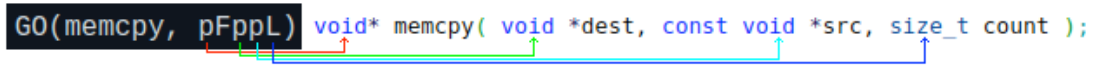
\includegraphics[width=\textwidth]{img/box64_sig.png}
	\caption{Пример сигнатуры функции memcpy}
	\label{fig:box64sig}
\end{figure}

После определения функция заносится в таблицу функций библиотеки, а затем находится при помощи разных методов. (// посмотреть что за методы (а надо?)).

Одной из оптимизаций в box64, по сравнению с box86 (32-х битной версией эмулятора), является определение простых функций, такие функции не нуждаются в оберточной функции и вызываются напрямую, тем самым экономя время.  \cite{box64_deep}

\subsubsection{Поддержка самомодифицирующегося кода}

I'm doing something similar, yes. All pages from which x86 code has been translated are write protected. Once a write occurs, all blocks generated from this page are marked dirty, and the jump table from those blocks are invalidated (to avoid automatic jump from block to block to this one). Once x86 code wants to run a "dirty" block, a crc32 of the memory is runned and compared to the crc computed when creating the block. depending if it's the same or non, the block is marked as clean (and the page protected again) or deleted and a new one is generated (and the page also protected again)

\subsection{FEX}

FEX это еще круче чем box и почему.

FEX, так же как и box64, является эмулятором пользовательского режима.

В FEX реализованы инструкции x86, x86-64, x87, mmx, sse1, sse2, sse3, ssse3 и bmi.

Трансляция происходит в 4 этапа:

\begin{itemize}[leftmargin=1.6\parindent]
	\item[---] Frontend: Декодирование инструкций, при декодировании также определяются границы блоков трансляции и функций;
	\item[---] OpDispatcher: Перевод инструкций во внутренние (SSA IR, IR.json) инструкции;
	\item[---] IR/Passes: Оптимизация внутренних инструкций;
	\item[---] JIT: Трансляция внутренних инструкций.
\end{itemize}

\subsection{Frontend}
Инструкции x86 декодируются в более простые для обработки, например инструкция add имеет большое количество разных опкодов, хотя по своей сути там меняются размеры и типы операндов, а не сама операция. Тогда операции add декодируются как:
\texttt{
\\
00 C0: add al ,al  \\
04 01: add al, 0x1 \\}
таким образом попадая в одну категорию.

Именно Frontend разбивает код на блоки трансляции. Рассматривается ситуация когда блоки трансляции находятся в одном месте. Некоторые трансляторы заканчивают трансляцию при любой потере управления, хотя в скомпилированном коде часто встречаются такие конструкции:
\texttt{
\\
test eax, eax\\
jne .Continue\\
ret           <--- Можно продолжать трансляцию после безусловной потери управления\\
.Continue:\\
}

Если можно определить адрес условного перехода, то есть возможность продолжить трансляцию.

\subsection{OpDispatcher}

Внутри FEX используется промежуточное представление, эти команды напоминают ARM64. Так как набор различных инструкций x86 слишком велик (более 1000) предлагается сначала переводить их в IR, а затем оптимизировать. На этом этапе обрабатываются особенности x86 (например MOVSB и подобные инструкции разворачиваются в циклы). OpDispatcher не выделяет регистры. 

\subsubsection{IR SSA}

После трансляции в IR количество инструкций больше изначального в 10-30 раз. 32-х битные инструкции расширяются до 64 бит.

\subsection{IR/Passes}

На этом шаге применяются разные методики для оптимизации инструкций.

\subsubsection{Распространение констант (ConstProp)}
При этом проходе заменяется выражение, которое при выполнении всегда возвращает одну и ту же константу, самой этой константой. Это значение прописывается в инструкцию.

\subsubsection{Устранение мертвого кода (DeadCodeElimination)}
Устраняется бессмысленный, не вызываемый код.

\subsubsection{Устранение загрузок контекста (DeadContextStoreElimination)}
Устраняются бесполезные загрузки контекста, например если идет сохранение контекста, а затем сразу же его загрузка, такая загрузка выполнятся не будет. 

\subsubsection{Устранение хранения (DeadStoreElimination)}
Устраняются бесполезные хранения, не высчитываются неиспользуемые флаги (например, те что будут перезаписаны следующей инструкцией: при операции умножения или деления используют несколько регистров и один из этих регистров будет перезаписан следующей инструкцией), устраняются бессмысленные и ненужные операции, так же как в QEMU.

Еще пример, если после ветвления в любом случае перезаписывается какое-либо значение — его можно не хранить.

\subsubsection{Сжатие инструкций (IRCompaction)}
Многие x86 инструкции читают или записывают регистры подряд, можно объединять их в пары (и использовать ld2 или st1 и подобные).

Некоторые MMX операции (то есть с операндами в 64 бита) можно объединить в операции с операндами в 128 бит.

\subsubsection{Long divide removal pass}
Посоветоваться. (там шок может мне ашот расскажет)

\subsubsection{RedundantFlagCalculationElimination}

\subsubsection{Static register allocation}
На ARM можно использовать регистровый файл, если все правильно определить регистры можно заменять store context на store registers (уточнить (может это вообще не оптимизация)).

\subsubsection{Устранение временных регистров}
Если транслируется блок который включает в себя весь код функции и известен используемый двоичный интерфейс можно исключить временные регистры при сохранении контекста. Также при трансляции целой функции можно убрать загрузки и сохранения в контекст посреди функции и выполнять одно сохранение в конце функции и загрузку в начале.

\subsubsection{Block chaining}
Та же идея что и в qemu, таким образом сильно снижается время поиска следующего блока при безусловном ветвлении.

\subsection{Трансляция IR в инструкции хоста, JIT}

При трансляции также используется кэш, для каждого потока кэш свой что приводит к избыточности, зато нет проблемы синхронизации. (это шок вообще мне надо писать про организацию кэшей в FEX?)
И еще есть LookupCache, это адреса? (вроде)
(External/FEXCore/Source/Interface/Core/LookupCache.cpp, используется в Arm64Dispatcher.cpp)

Третий уровень используется для реконструкции второго уровня в случае переполнения. Первый уровень не переполняется (разработчик так говорит).

\subsection{Поддержка самомодифицируещегося кода.}
Полноценной поддержки нет, автор считает что подход QEMU и box64 является единственным приемлемым по скорости и хочет использовать его.

\begin{comment}
\subsection{ДАЛЬШЕ МОЖНО НЕ ЧИТАТЬ}

Список:

\begin{itemize}[leftmargin=1.6\parindent]
	\item[---] первое;
	\item[---] второе;
	\item[---] пятое;
	\item[---] десятое.
\end{itemize}

Формула:

\begin{equation}
c^2 = a^2 + b^2
\end{equation}

Ссылаемся на рисунок \ref{fig:a1}. Информация из источника \cite{golang}.

\begin{figure}[hbtp]
	\centering
	
\includegraphics[width=\textwidth]{img/golang.png}
	\caption{Пример рисунка}
	\label{fig:a1}
\end{figure}

\begin{code}
	\captionof{listing}{Пример кода}
	\label{code:1}
	\inputminted
	[
	frame=single,
	framerule=0.5pt,
	framesep=20pt,
	fontsize=\small,
	tabsize=4,
	linenos,
	numbersep=5pt,
	xleftmargin=10pt,
	]
	{text}
	{code/main.go}
\end{code}
\end{comment}

\pagebreak